\chapter{iHome Charging}

Visando a preocupação em oferecer uma altamente sustentável e a melhoria na qualidade de vida, deve-se estender essa atenção para os meios de transporte utilizados pela família, a sustentabilidade deve existir, também, no estilo de vida das pessoas que irão morar em nossa casa. De nada adianta morar em uma casa sustentável e adotar uma forma de viver que seja prejudicial ao meio ambiente. Partindo deste princípio, foi obtida a ideia de implementar em nosso projeto um carro híbrido (motor à combustão e elétrico) e uma garagem que carregue as suas baterias enquanto o carro estiver estacionado.

\begin{figure}[H]
\begin{center}
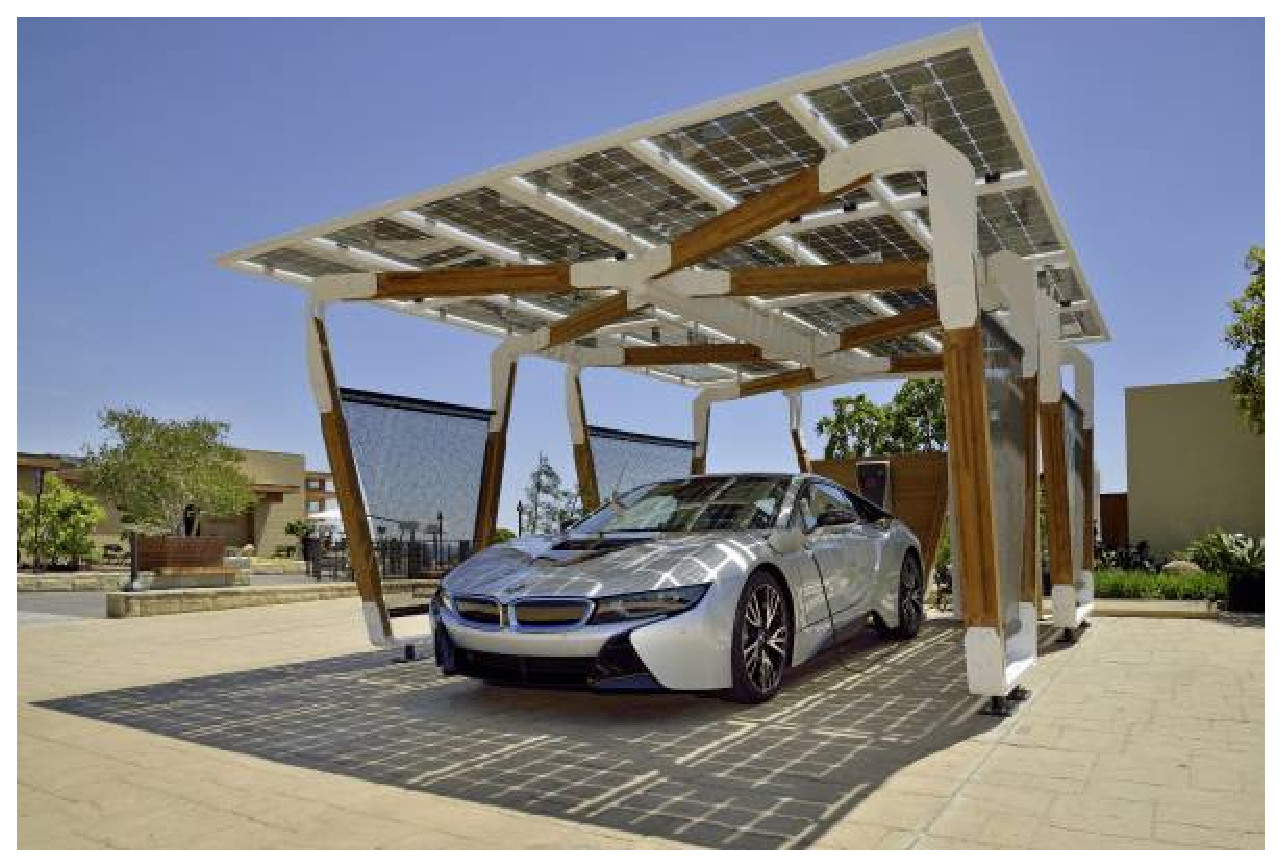
\includegraphics[keepaspectratio,scale=0.6]{figuras/ihomecharging.jpg.eps}
\caption{iHome Charging}
\end{center}
\end{figure}

Este é um sistema desenvolvido pela BMW, no qual aproveita 25 metros quadrados de painéis solares dispostos no teto da garagem, para que esta energia seja reaproveitada carregando as baterias do carro, estes 25 metros quadrados podem produzir, por ano, o suficiente para um alcance por volta de 32000 quilômetros, isto é mais que o bastante para um cidadão que usa o seu carro para ir e voltar do trabalho todos os dias, na maioria dos casos. Na falta da energia solar, ou quando ela não for suficiente para abastecer totalmente o carro, a garagem carrega as baterias do carro apenas em horários que a energia é mais barata, o que chamamos no Brasil de tarifa branca. Durante o dia, por exemplo, a energia é mais barata, pois o uso dela não é muito requisitado, diferente do início da noite, onde a demanda energética atinge o seu pico.

\section{Carro compatível com a proposta da casa}
\subsection{BMW i8}

\begin{figure}[H]
\begin{center}
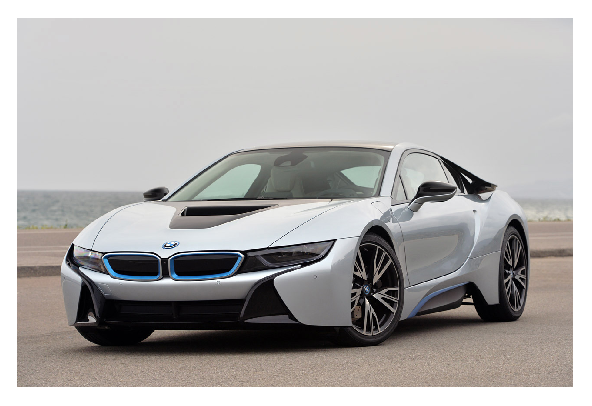
\includegraphics[keepaspectratio,scale=0.8]{figuras/bmwi8.jpg.eps}
\caption{BMW i8}
\end{center}
\end{figure}

Este carro tem espaço para 4 ocupantes e vai de 0-100 \nicefrac{\si{\kilo\meter}}{\si{\hour}} em apenas 4,4 segundos. Sua carroceria é feita de fibra de carbono, cerca de 50\% mais leve do que o aço e cerca de 30\% mais leve do que o alumínio, porém igualmente estável e resistente. Este material serve para compensar o peso das baterias, o que dá a este carro um peso final de 1490\si{\kilo\gram}. O motor elétrico é alimentado por baterias de Íons de Lítio com alta voltagem de 5\si{\kilo\watt\hour}. Seu pack de baterias tem a capacidade de armazenar 266\si{\kilo\watt} de energia. O consumo médio é de 2,5\si{\liter}/100\si{\kilo\meter} e tem 35\si{\kilo\meter} de autonomia em modo elétrico – com o qual pode atingir velocidades até 120\nicefrac{\si{\kilo\meter}}{\si{\hour}} - e 500 \si{\kilo\meter} de alcance em configuração híbrida.

Com todos esses números, não é de se esperar um preço muito acessível.

\begin{figure}[H]
\begin{center}
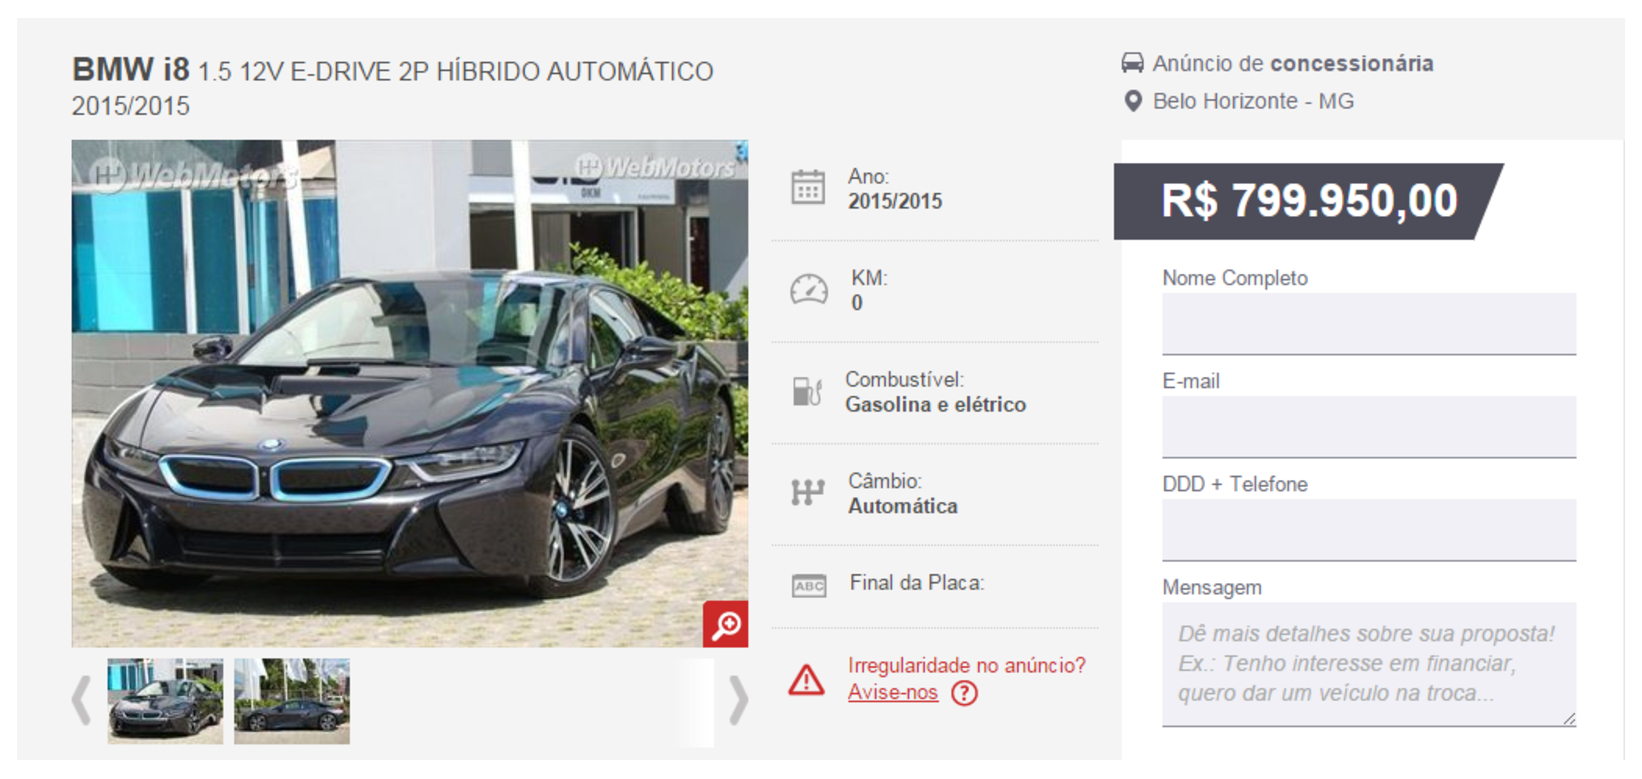
\includegraphics[keepaspectratio,scale=0.4]{figuras/bmwi8preco.eps}
\caption{Preço do BMW i8}
\end{center}
\end{figure}

\subsection{BMW i3}

\begin{figure}[H]
\begin{center}
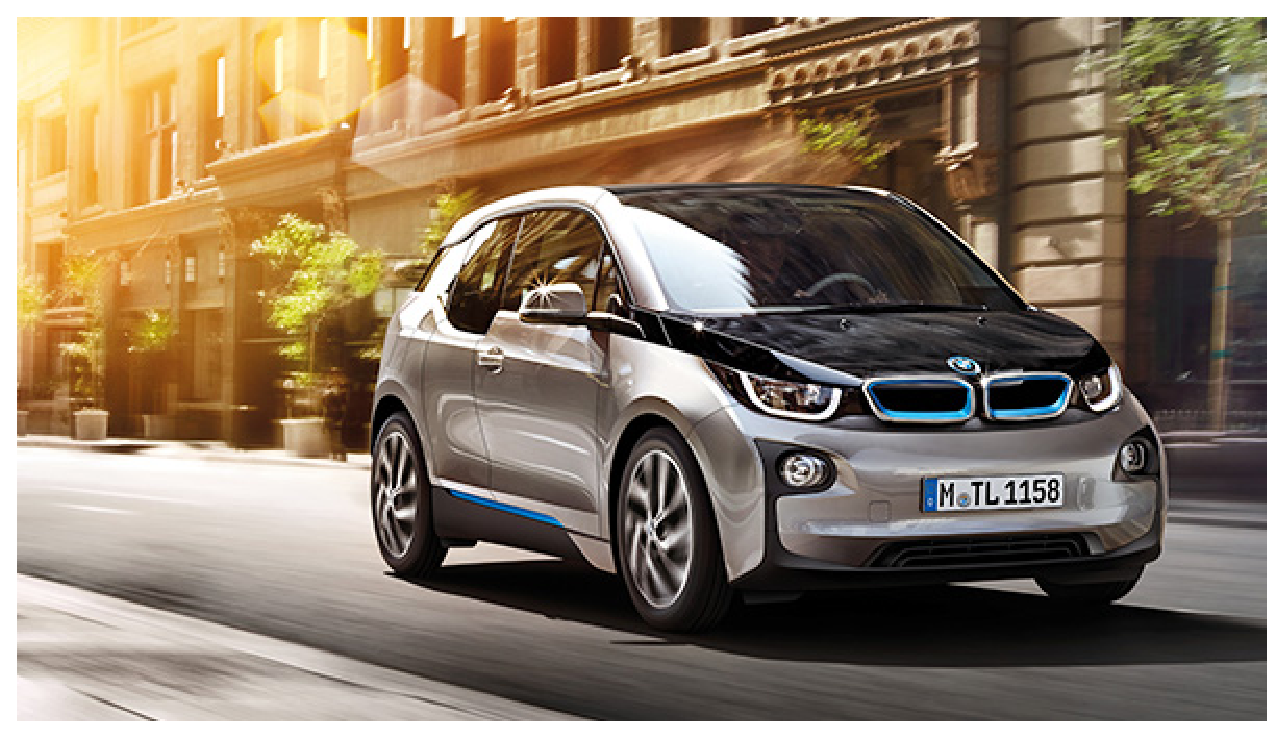
\includegraphics[keepaspectratio,scale=0.5]{figuras/i3.jpg.eps}
\caption{BMW i3}
\end{center}
\end{figure}

Este carro tem espaço para 4 ocupantes e vai de 0-100\nicefrac{\si{\kilo\meter}}{\si{\hour}} em apenas 7,2 segundos. A preocupação com o meio ambiente parte desde a construção do veículo, sua carroceria é feita de fibra de carbono e alumínio através de máquinas que utilizam energia provenientes de fontes renováveis, o interior é composto por 25\% de plástico reciclado. A junção de todos estes materiais dá ao carro um peso final de 1390\si{\kilo\gram}. O motor elétrico é alimentado por baterias de Íons de Lítio capazes de armazenar 125\si{\kilo\watt} de energia. O alcance deste carro com a bateria carregada é de 170\si{\kilo\meter}.

\begin{figure}[H]
\begin{center}
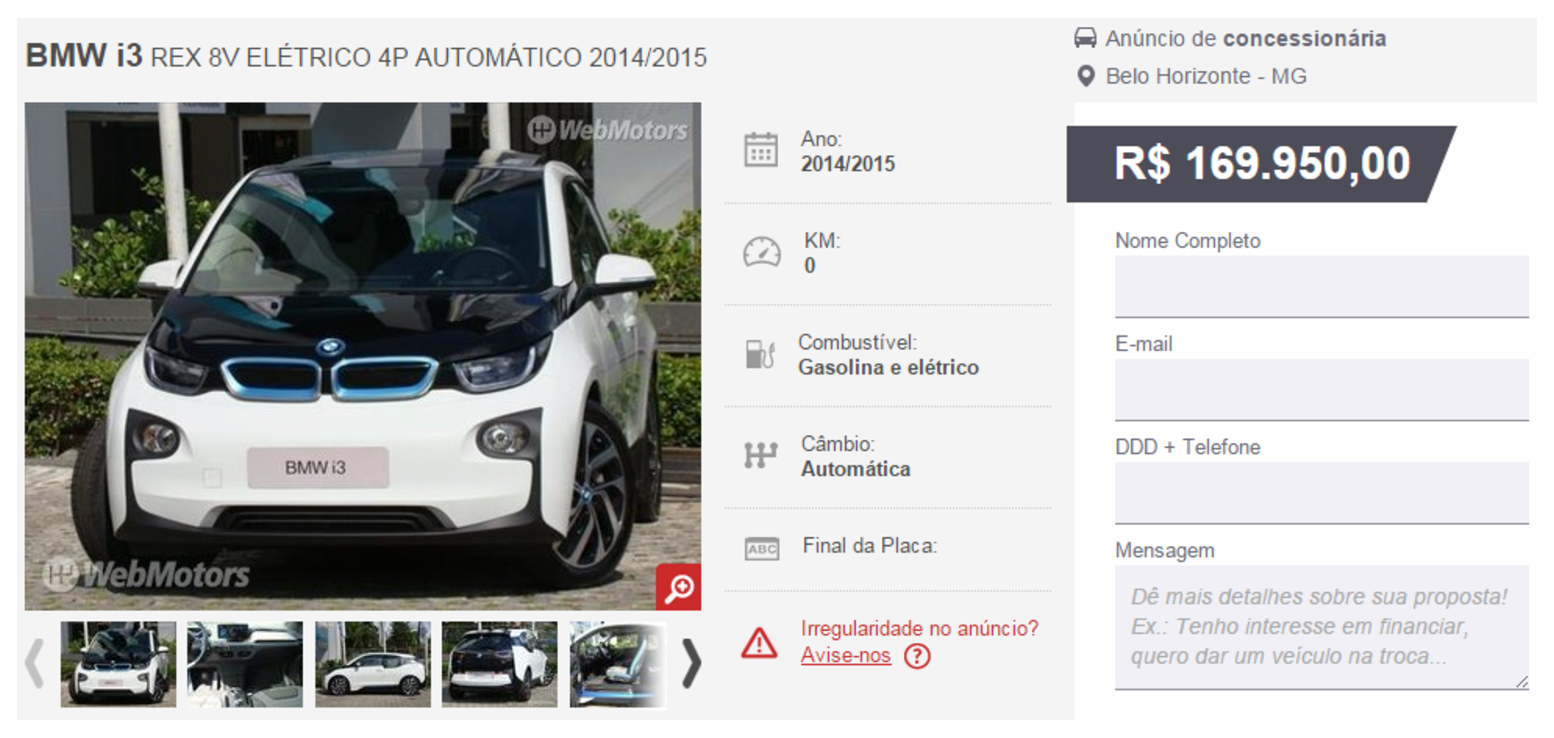
\includegraphics[keepaspectratio,scale=0.5]{figuras/i3preco.eps}
\caption{Preço do BMW i3}
\end{center}
\end{figure}

\subsection{Fusion Hybrid}

\begin{figure}[H]
\begin{center}
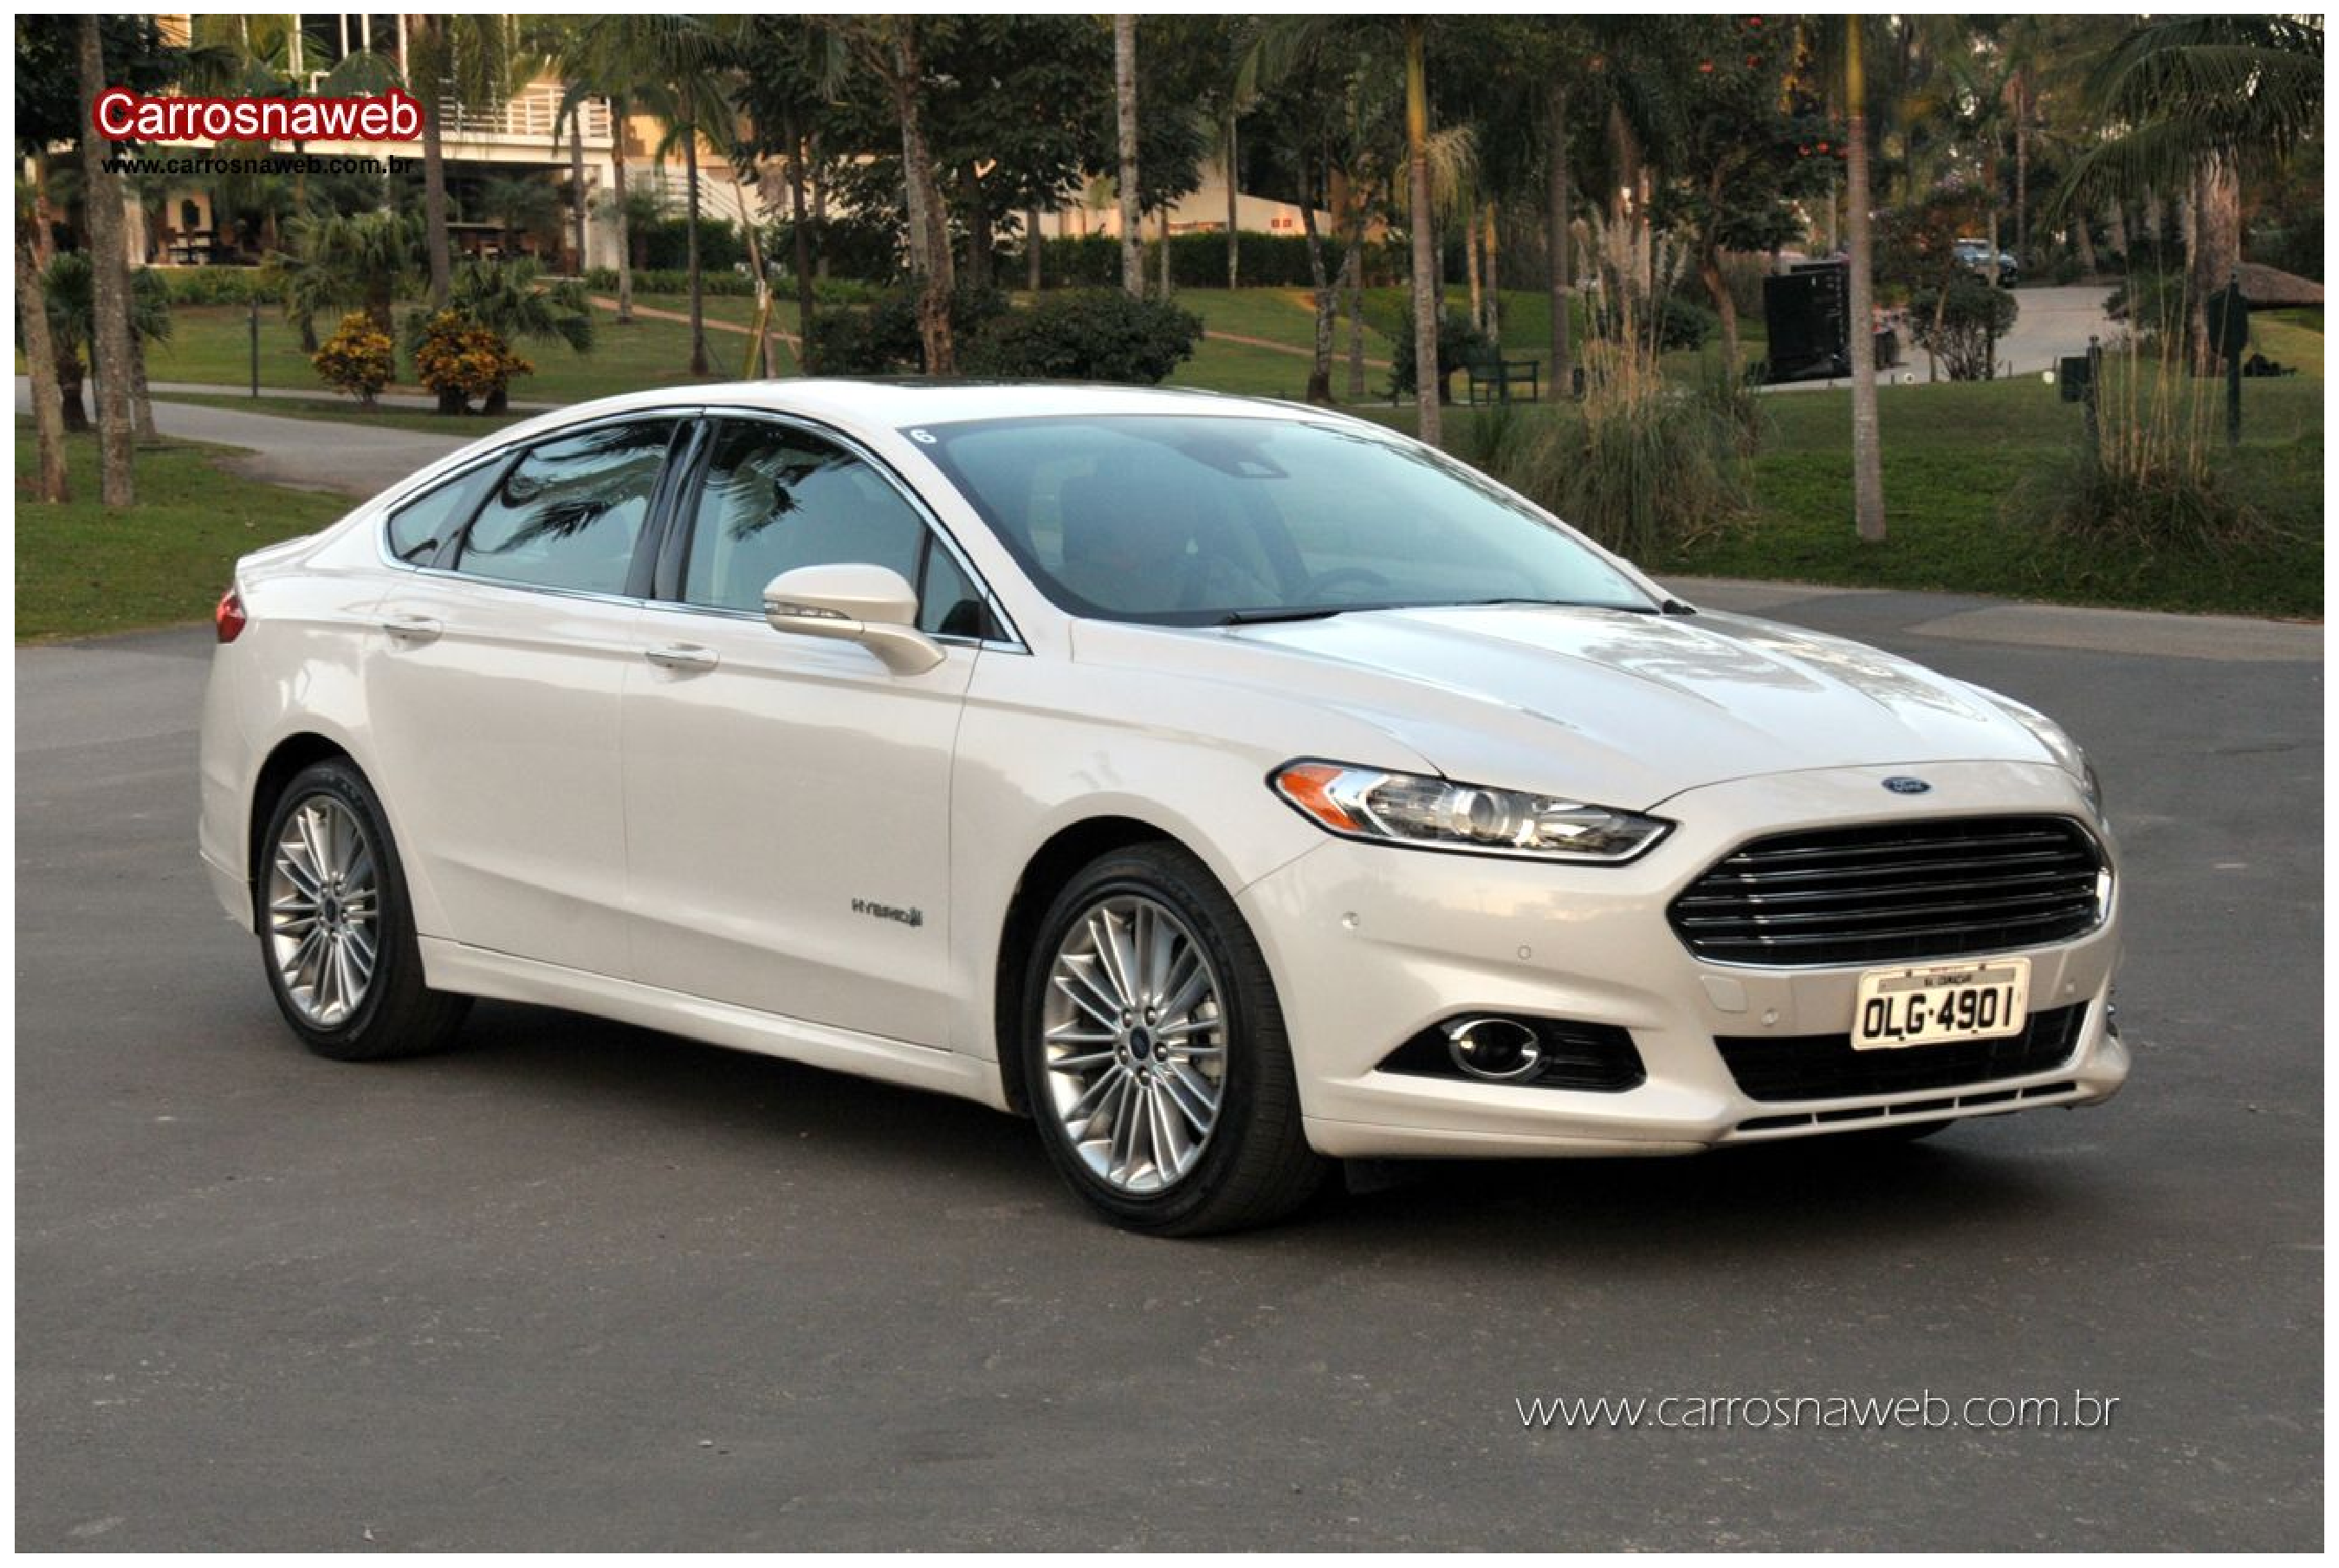
\includegraphics[keepaspectratio,scale=0.15]{figuras/fusion.eps}
\caption{Fusion Hybrid}
\end{center}
\end{figure}


Este carro tem espaço para 5 ocupantes e vai de 0-100 \nicefrac{\si{\kilo\meter}}{\si{\hour}} em 9,3 segundos. Ele pesa 1717 \si{\kilo\gram}. O motor elétrico é alimentado por baterias de Íons de Lítio capazes de armazenar 88\si{\kilo\watt} de energia. O consumo deste carro é, em média 16,8 \nicefrac{\si{\kilo\meter}}{\si{\liter}}.


\begin{figure}[H]
\begin{center}
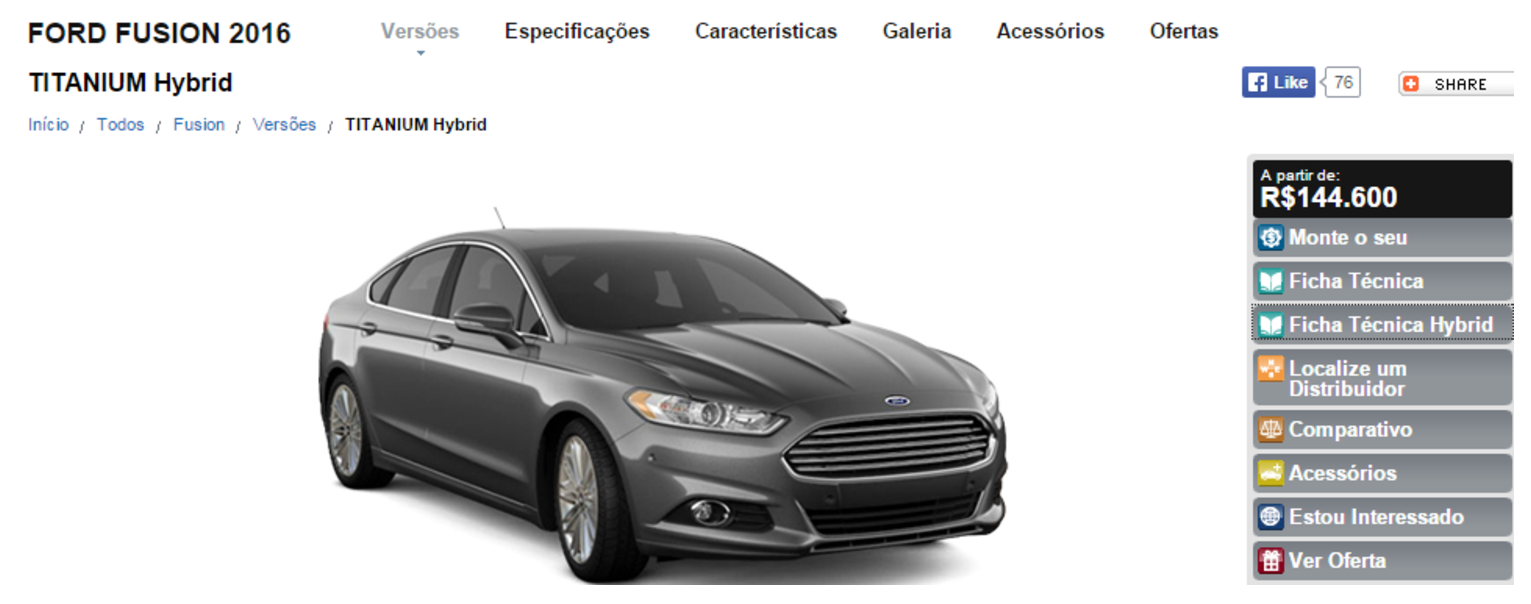
\includegraphics[keepaspectratio,scale=0.5]{figuras/fusionpreco.eps}
\caption{Preço do Fusion Hybrid}
\end{center}
\end{figure}

\section{Conclusão}

Após a análise de todos os carros, conclui-se que o i3 se encaixa melhor em no projeto, cabe exatamente o número de pessoas que haverá na casa. Apesar do Fusion Hybrid ser mais espaçoso, a Ford não se preocupou tanto quanto a BMW na escolha de materiais para inserir em seu projeto, isto resultou em um carro pesado e que, apesar de ser híbrido, não tem um consumo que encha tanto os olhos como é de se esperar. O BMW i8 esbanja potência e preço, seria uma alternativa muito luxuosa. Já que em Brasília, a qualidade de nossas estradas e a fiscalização não permite que essa potência seja totalmente explorada, o i8 torna-se um gasto desnecessário para este caso. O i3 é puramente elétrico, independente de combustível fóssil para a locomoção, e tem um alcance considerável, 170km, este valor é mais do que suficiente para um uso diário do carro dentro da cidade.